\section{What is the LSDF-Portal}

% \begin{frame}[c]{TODOS}
%     \todo{Write mail: Deployment (version updates, installs, constrain to django3} \\
%       Test if updates to Project details require lessening timeframe. Write command?
%     \todo{Write Changelog} \\
%     \todo{Implement last features: publications sortable, command with mail on end\_date near} \\
% \end{frame}


\subsection{Overview}

\begin{frame}[c,fragile]{What is the LSDF-Portal?}
    \large
    \begin{itemize}[<+(1)->]
        \item LSDF-Portal: {\em administration} of storage projects
            \begin{itemize}[<+(1)->]
                % \item Based on Python/Django (more on that later)
                \item Research groups can request storage capacity for research projects
                \item Allows for {\em structured interaction} with admins
                \item {\em Transparent communication} of project status
                \item Created and improved over multiple SCC-internships
            \end{itemize}
        % \item Internally available at \url{https://lsdf.kit.edu}
        \item Internally available at: \url{https://www.lsdf.kit.edu/os/storageprojects/}
        \item Service description: \url{https://www.scc.kit.edu/dienste/11228.php}
        % \item Test instance available at \url{https://lsdf.fkarg.de}
        %     \begin{itemize}[<+(1)->]
        %         \item Play around with \verb!user:test! or \verb!admin4:lsdf! (both admin)
        %         \item (Cannot properly route from within KIT for some reason)
        %     \end{itemize}
    \end{itemize}
\end{frame}

\begin{frame}[c]{Project Lifecycle}
    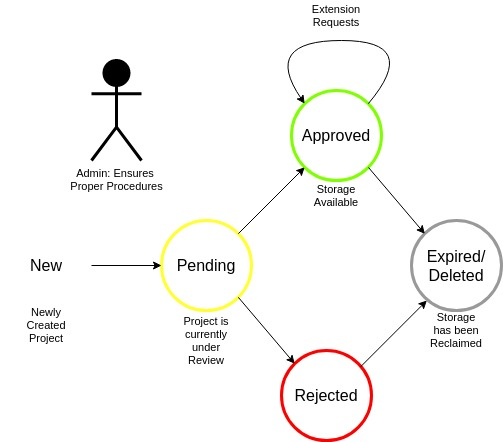
\includegraphics[height=0.9\textheight,center]{lsdf_states}
    % \todo{flash again on extension requests with them highlighted}
\end{frame}

% \begin{frame}[c]
%     \todo{tell story: maths requesting storage for digitalization?}
% \end{frame}
\subsection{Screenshots}


\addtocounter{framenumber}{1}
\begin{frame}[standout]
    \Huge
    Live Demo!
\end{frame}


\begin{frame}[c]{After First Login}
                           % trim=left bottom right top, clip
    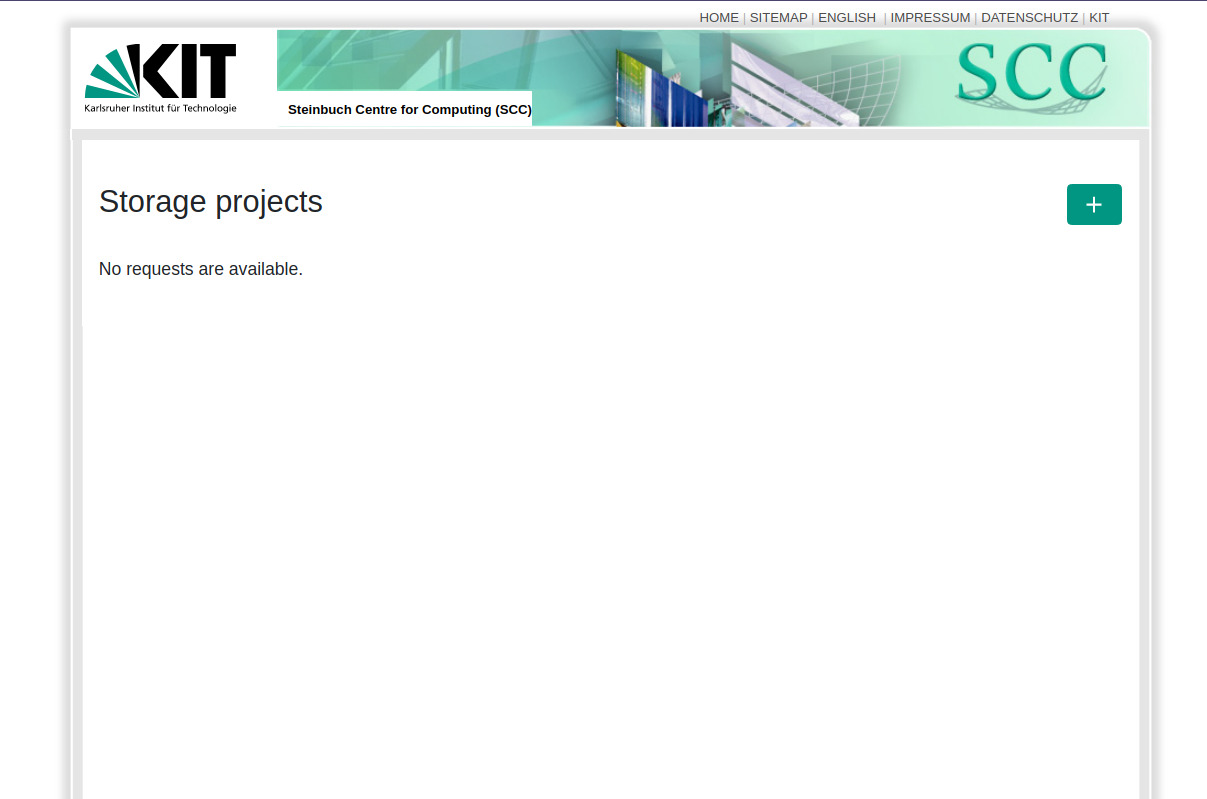
\includegraphics[width=\textwidth,trim=0 0 0 3,clip]{Selection_006}
\end{frame}

\begin{frame}[c]{Project Creation}
                           % trim=left bottom right top, clip
    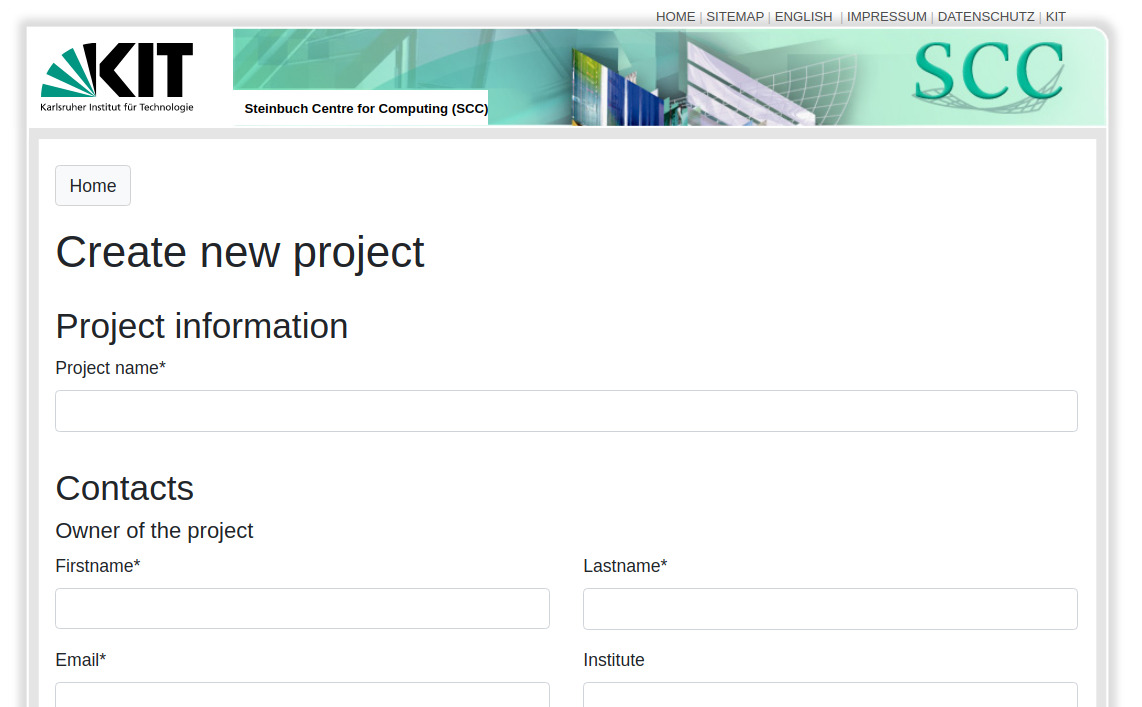
\includegraphics[width=\textwidth,trim=0 0 0 3,clip]{Selection_007}
\end{frame}

\begin{frame}[c]{Project Creation: Add Contacts}
                           % trim=left bottom right top, clip
    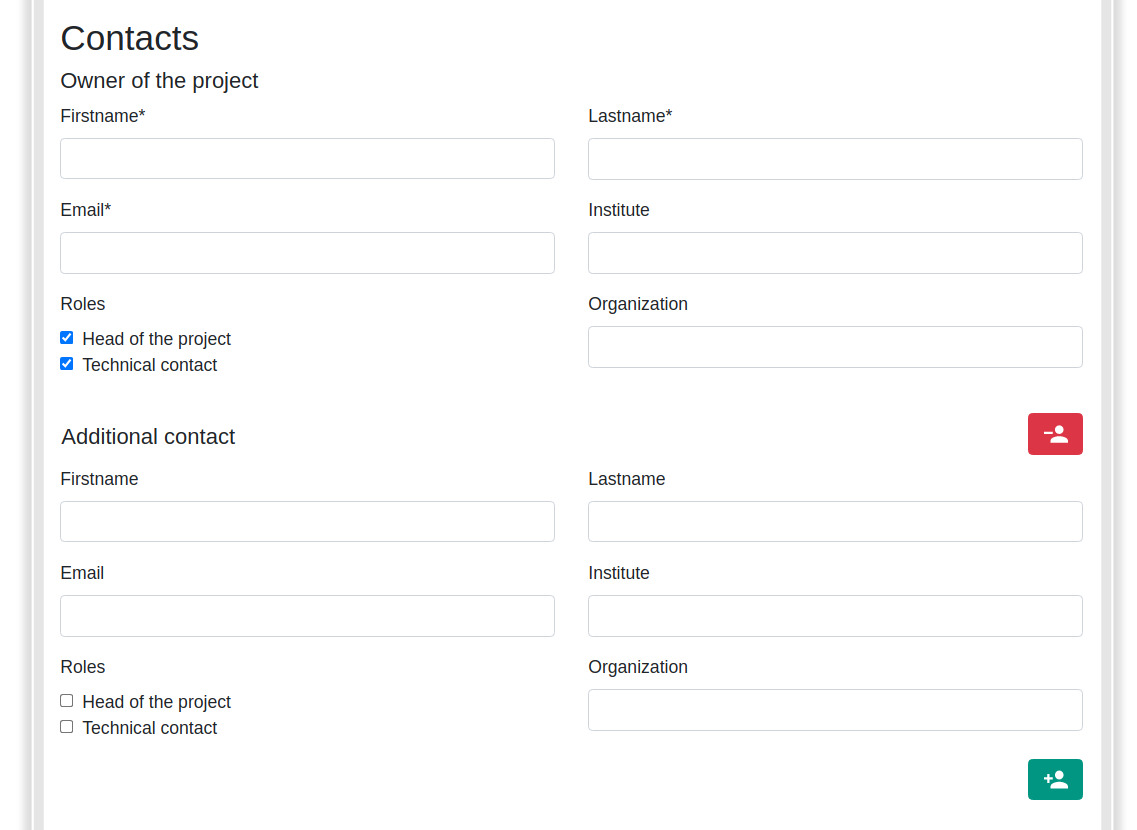
\includegraphics[width=\textwidth,trim=0 0 0 3,clip]{Selection_008}
\end{frame}

\begin{frame}[c]{Available Fields}
                           % trim=left bottom right top, clip
    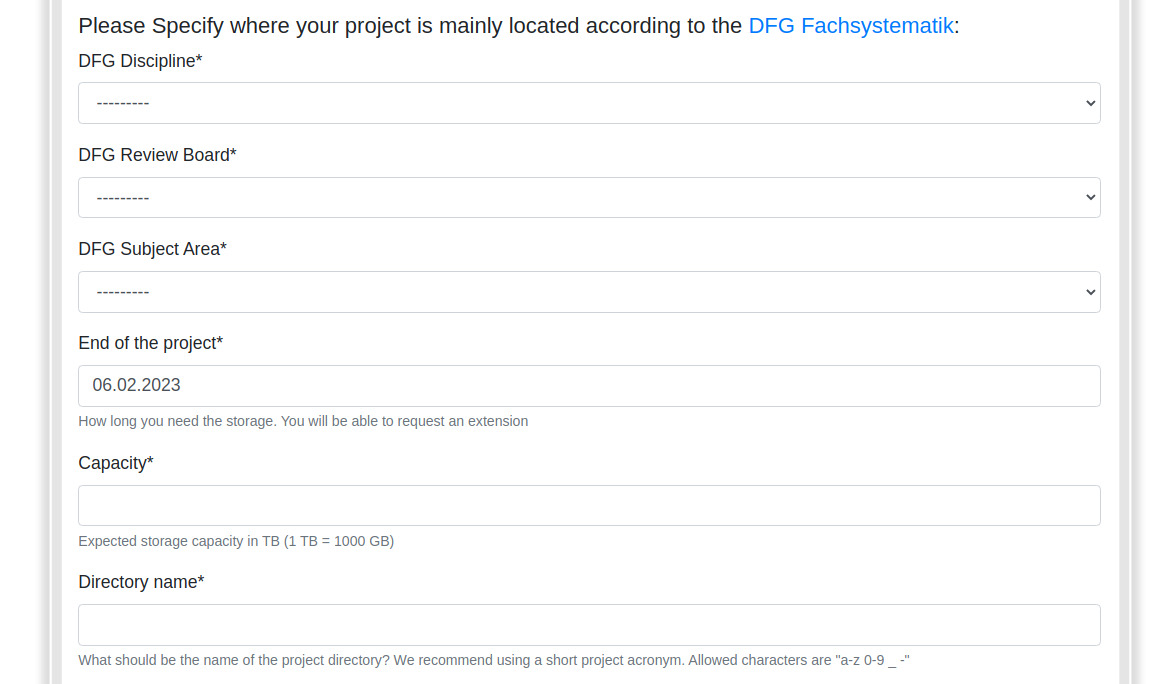
\includegraphics[width=\textwidth,trim=0 0 0 3,clip]{Selection_010}
\end{frame}

\begin{frame}[c]{Fields filled out}
                           % trim=left bottom right top, clip
    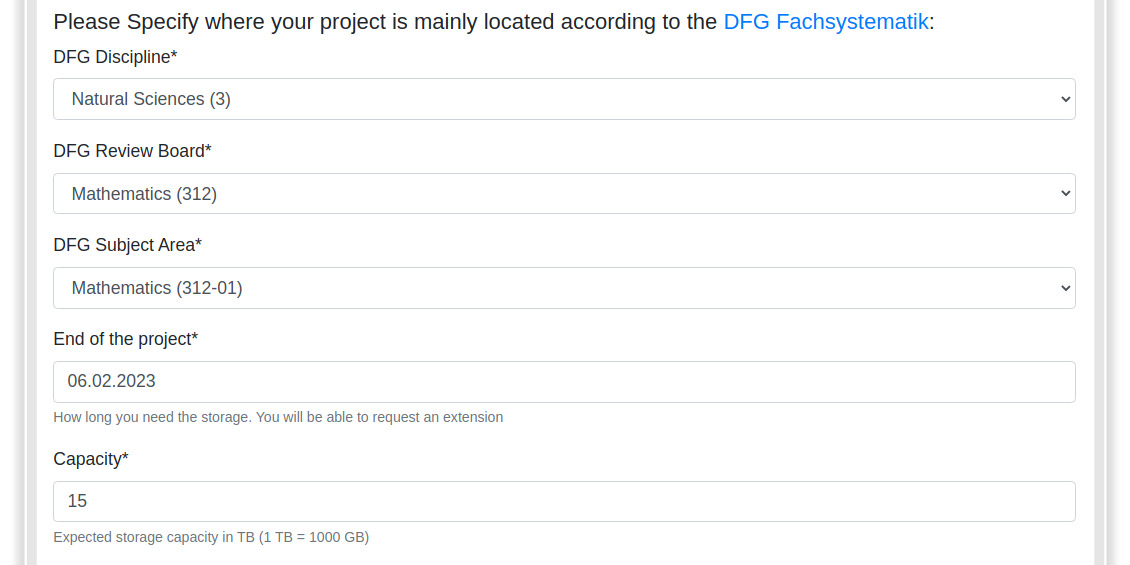
\includegraphics[width=\textwidth,trim=0 0 0 3,clip]{Selection_011}
\end{frame}

\begin{frame}[c]{Submit Proposal}
                           % trim=left bottom right top, clip
    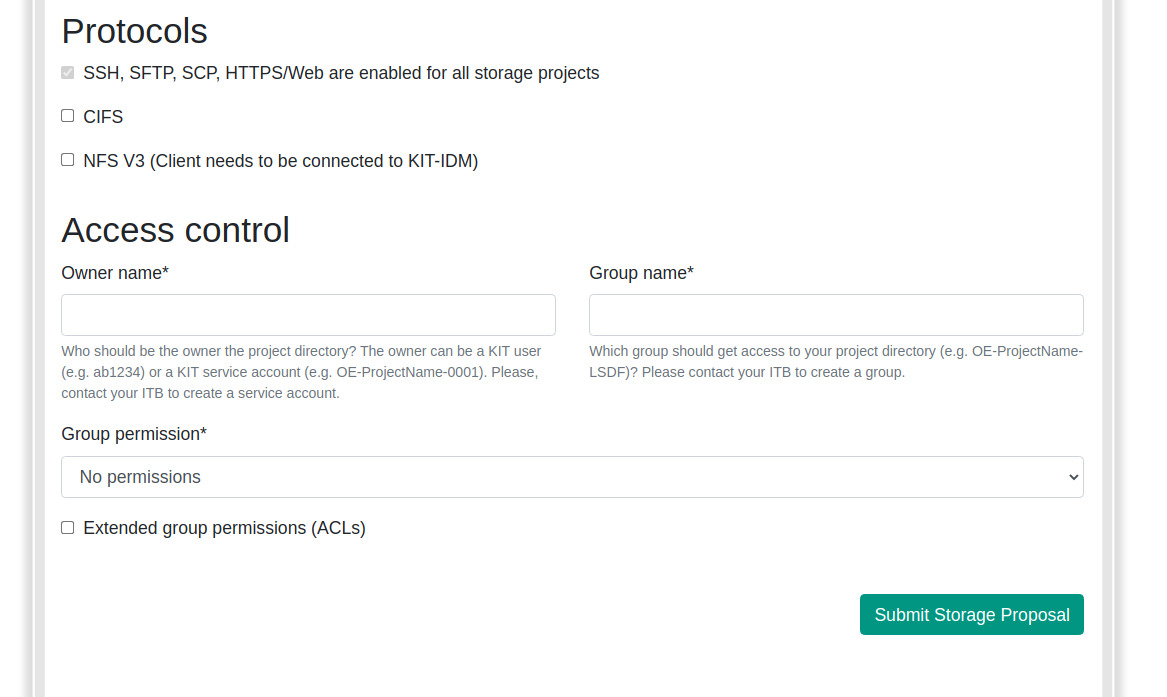
\includegraphics[width=\textwidth,trim=0 0 0 3,clip]{Selection_009}
\end{frame}

\begin{frame}[c]{Succesful Submission}
                           % trim=left bottom right top, clip
    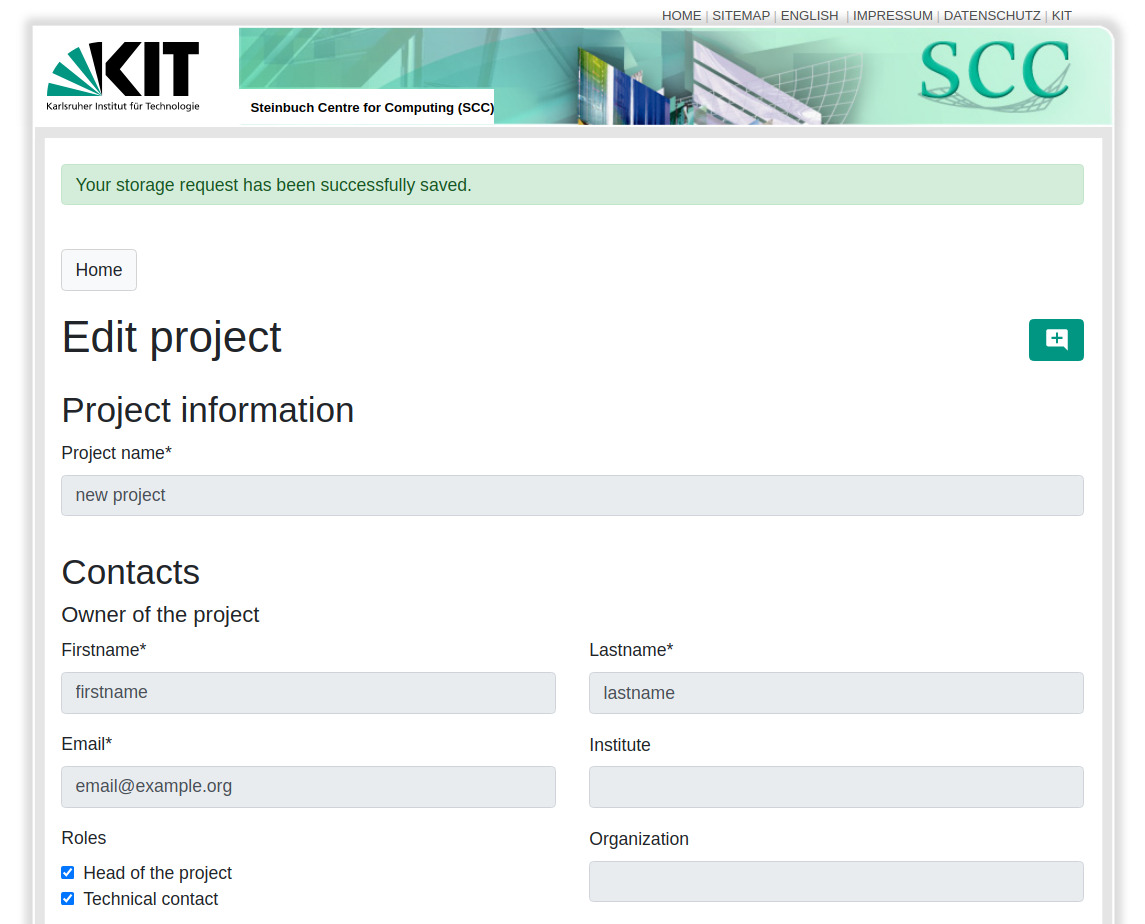
\includegraphics[width=\textwidth,trim=0 0 0 3,clip]{Selection_012}
\end{frame}

\begin{frame}[c]{Project in List}
                           % trim=left bottom right top, clip
    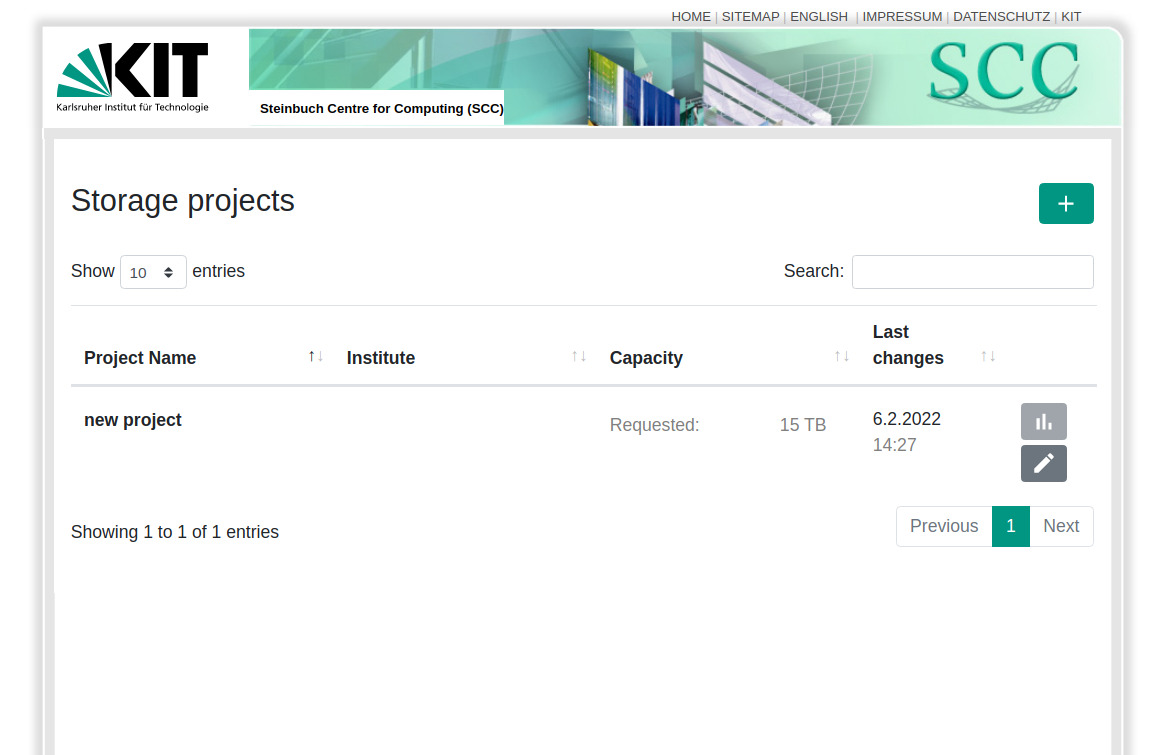
\includegraphics[width=\textwidth,trim=0 0 0 3,clip]{Selection_013}
\end{frame}

\begin{frame}[c]{Storage Use Histogram}
    \begin{center}
    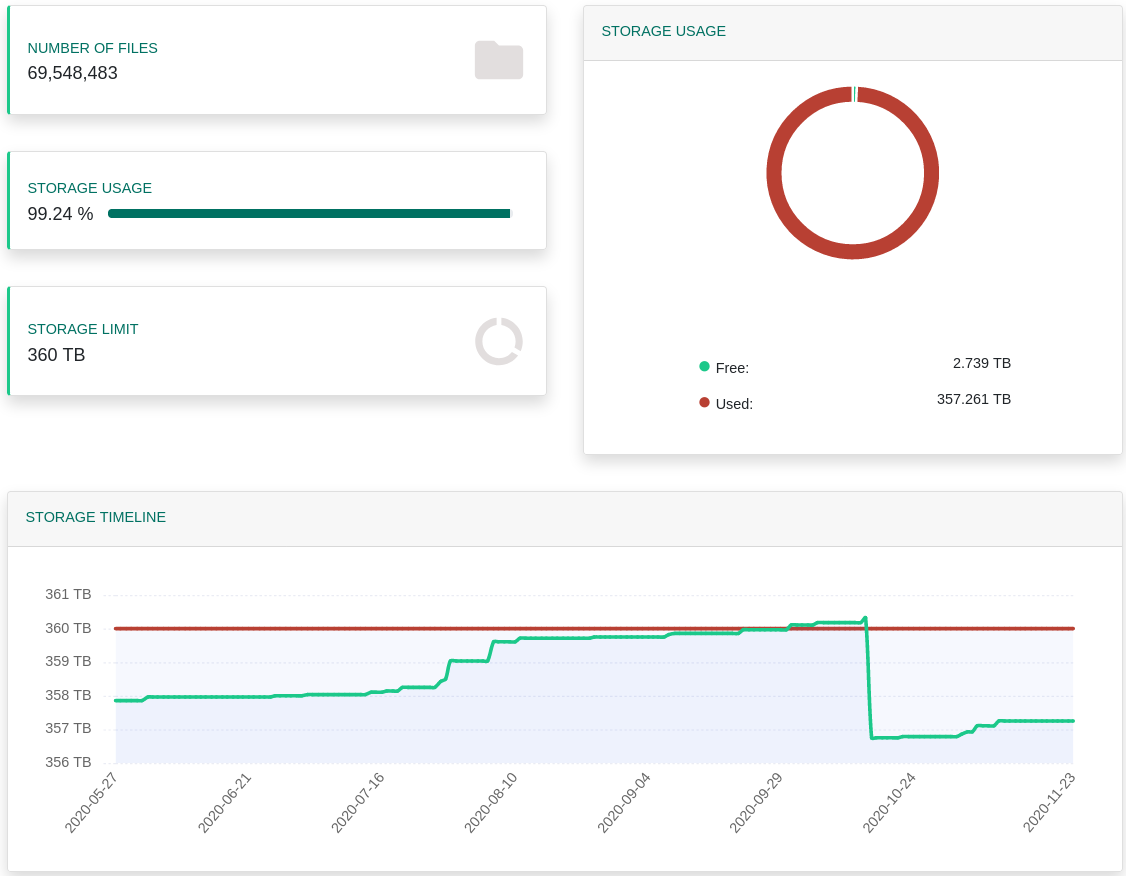
\includegraphics[height=\textheight]{lsdf-portal-usage}
    \end{center}
\end{frame}
